\documentclass[a4paper,12pt]{article}
\usepackage[utf8]{inputenc}
\usepackage[T1]{fontenc}

\usepackage[left=1.5cm, right=1.5cm, top=2cm, bottom=2cm, twoside]{geometry}

\usepackage{esvect}
\usepackage{siunitx}
\usepackage{fancybox}

\usepackage{amsmath}
\usepackage{amsfonts}
\usepackage{amssymb}
\usepackage{amsthm}

\usepackage{braket}
\usepackage{graphicx}
\usepackage{mathptmx}
%\usepackage{tikz}
\usepackage{pgfplots}
\usepackage{siunitx}
\usepackage{hyperref}


\usepackage{pstricks}
\usepackage{pstricks-add}
\usepackage{pst-plot}
\pgfplotsset{compat=1.17}

\usepackage[french]{babel}
%Raccourcis de la flemme
\newcommand{\R}{\mathbb{R}}
%\newcommand{\C}{\mathbb{C}}
\newcommand{\D}{\, \mbox{d}}

\hypersetup{
 pdfauthor={Tanneguy Blandin},
 pdftitle={Devoir maison: Physique du solide},
 pdfkeywords={},
 pdfsubject={},
 pdfcreator={Me}, 
 pdflang={French}}

%Définition des numéros d'éxercices
\newcounter{numExo}
\newcounter{partExo}
\newcounter{numQuestion}
\newcounter{numSubQuestion}


\newcommand{\exercice}[1]{%
  \stepcounter{numExo}%
  \setcounter{partExo}{0}%
  \setcounter{numQuestion}{0}%
  \setcounter{numSubQuestion}{0}%
    \noindent
    \section*{Exercice \arabic{numExo}: #1}
    \addcontentsline{toc}{section}{\protect\numberline{}Exercice \arabic{numExo}: #1}
}
\newcommand{\partexo}[1]{%
  \stepcounter{partExo}%
    \setcounter{numQuestion}{0}%
    \setcounter{numSubQuestion}{0}%
    \noindent
    \subsection*{\Alph{partExo} -- #1}
    \addcontentsline{toc}{subsection}{\protect\numberline{}\Alph{partExo}: #1}
    }

\newcommand{\Question}{%
  \stepcounter{numQuestion}%
  \setcounter{numSubQuestion}{0}%
 \par\noindent \textbf{\arabic{numQuestion}.\hspace{2pt}}}


\newenvironment{question}%
{%
\ttfamily %
  \stepcounter{numQuestion}%
  \setcounter{numSubQuestion}{0}%
 \par\noindent \textbf{\arabic{numQuestion}}
}%
{%
\normalfont
}

\newenvironment{info}%
{%
\ttfamily %
}%
{%
\normalfont
}

\newcommand{\subquestion}{%
  \stepcounter{numSubQuestion}%
  \par{}\hspace{3pt}\textbf{\arabic{numSubQuestion}.\hspace{2pt}}}


%%INFO DOC
\title{Devoir maison \\ Physique des matériaux \\ \large{\textsc{insa} Rennes -- 3 SGM}}
\date{Mars 2021}
\author{Tanneguy Blandin}

  
\begin{document}
\maketitle


\exercice{Cristal bidimensionnel}

\partexo{Réseau}

\begin{figure}[htb]
  \centering
  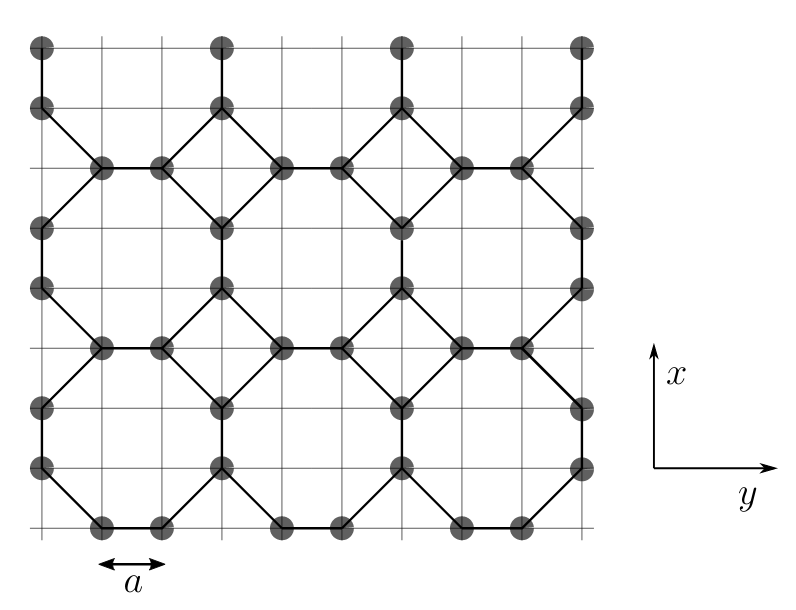
\includegraphics[width=0.5\textwidth]{./pictures/cristal2D.png}
  \caption{Cristal 2D}
  \label{fig:cristal2D}
\end{figure}

\begin{question}
  Donner les coordonnées des vecteurs $(\vv{a},\vv{b})$ qui définissent une maille primitive de ce réseau dans le repère $Oxy$ orthonormé, en fonction de $a_0$.
\end{question}

La maille est une maille carrée, les vecteurs de la maille élémentaire de ce réseau sont $\vv{a}=(3a_0,0)$ et $\vv{b}=(0,3a_0)$. Cependant, la maille primitive
ne doit être consitué aue d'un unique noeud du réseau. AHHH

\begin{question}
  Préciser la nature du réseau direct et son paramètre de maille $a$
\end{question}



\begin{question}
  Préciser le motif associé à ce cristal : nombre d'atomes et position en fonction des vecteurs $\vv{a}$ et $\vv{b}$
\end{question}


\begin{question}
  Calculer l'aire de la maille unitaire, en fonction de $a_0$
\end{question}

\begin{question}
  Calculer le nombre d'atomes par unité de surface. Application numérique en \si{\squared\meter}.
  \end{question}

\begin{question}
  Exprimer les coordonnées des vecteurs du réseau réciproque $(\vv{a*}, \vv{b*})$, en fonction de $a_0$ dans le repère $Oxy$
\end{question}


\begin{question}
  Dessiner le réseau réciproque et le première zone de Brillouin
\end{question}
\begin{question}
  Dans la première zone de Brillouin, placer les points $\Gamma$ ,$X$ de coordonnées $(\pi/a,0)$ et $M$ de coordonnées $(\pi/a,\pi/a)$.
  \end{question}




\partexo{Bandes d'énergie}
\begin{info}
  On suppose que l'énergie des électrons de conduction est représentée par :
  \begin{equation}\label{equ:enerelectron}
    E_c(\vv{k})= \alpha  - 2 \gamma \left( \cos(k_x a)  + \cos(k_y a)    \right)
  \end{equation}
\end{info}


\Question En prenant l'équation~\ref{equ:enerelectron} pour définir l'énergie des électrons de conduction, nous pouvons calculer l'énergie aux points caractéristiques de la maille en prenant $\alpha = \SI{2,5}{\eV}$ et $\gamma = \SI{0,5}{\eV}$:
\begin{itemize}
\item En $\Gamma$ ($\vv{k}=(0,0)$), nous avons: $E_{c\Gamma} = \alpha - 4\gamma= \SI{0,5}{\eV}$.
\item En $X$ ($\vv{k}=(\pi/a,0)$), nous avons: $E_{cX} = \alpha = \SI{2,5}{\eV}$ .
\item En $M$ ($\vv{k}= (\pi/a,\pi/a)$), nous avons: $E_{cM} = \alpha + 4\gamma = \SI{4,5}{\eV}$.
\end{itemize}

\Question En déterminant la ou les composantes de $\vv{k}$ qui varie ou varient en fonction de la direction dans laquelle nous nous déplaçons dans le cristal, nous pouvons réécire la fonction $\vv{k}$ pour chaque direction:
\begin{itemize}
\item Sur la direction $\Gamma X$ ou $\Delta$, nous pouvons définir $\vv{k}$ en fonction de $x$ de la manière suivante:
  \begin{align*}
    [0,\frac{\pi}{a}] & \rightarrow [0,\frac{\pi}{a}]^2\\
    x                 & \mapsto    \vv{k} = (x,0) \\
  \end{align*}
  Nous pouvons donc définir la variation de l'énergie dans cette direction:
  \begin{equation}\label{equ:Delta}
    x\in[0,\frac{pi}{a}] \quad E_{c\Delta} = \alpha - 2\gamma\left(1+\cos(ax)\right)
  \end{equation}

\item Sur la direction $\Gamma M$, nous pouvons définir $\vv{k}$ en fonction de $x$x de la manière suivante:
  \begin{align*}
    [0,\frac{\pi}{a}] & \rightarrow [0,\frac{\pi}{a}]^2\\
    x                 & \mapsto    \vv{k} = (x,x) \\
  \end{align*}
  Nous pouvons donc définir la variation de l'énergie dans cette direction:
  \begin{equation}\label{equ:GammaX}
    x\in[0,\frac{pi}{a}] \quad E_{c\ \Gamma X} = \alpha - 4\gamma\cos(ax)
  \end{equation}

\item Sur la direction $XM$, nous pouvons aussi définir $\vv{k}$ en fonction de $x$:
  \begin{align*}
    [0,\frac{\pi}{a}] & \rightarrow [0,\frac{\pi}{a}]^2\\
    x                 & \mapsto    \vv{k} = (\frac{\pi}{a},x) \\
  \end{align*}
  Nous pouvons donc définir la variation de l'énergie dans cette direction:
  \begin{equation}\label{equ:XM}
    x\in[0,\frac{pi}{a}] \quad E_{c\ XM} = \alpha - 2\gamma(\cos(ax)-1)
  \end{equation}
\end{itemize}


Nous pouvons représenter l'évaluation de l'énergie en fonction de la position sur les principales directions, c'est que que nous faisons sur la figure

\begin{figure}[htb]
  \centering
  \begin{pspicture}(-4,-1)(7.14,5)
    \psline[showpoints=true, dotstyle=pentagon*](-3.14159,0)(0,0)(3.14159,0)(6.283185,0)
    \psline[showpoints=true, dotstyle=pentagon*]{->}(0,0)(0,1)(0,2)(0,3)(0,4)(0,5)
    %% M->Gamma
    \def\EMG{x RadtoDeg cos -2 mul 2.5 add}
    \psplot{-3.141592}{0}{\EMG}
%    \uput[d](-3,0){$M$}
    %% Gamma -> X
    \def\Delta{x RadtoDeg cos 1.5 sub neg}
    \psplot{0}{3.141519}{\Delta}
%    \uput[d](0,0){$\Gamma$}
    %% X -> M
    \def\EXM{x 3.141519 sub RadtoDeg cos -1 mul 3.5 add}
    \psplot{3.141519}{6.28318}{\EXM}
%    \uput[d](3.141592,0){$X$}
%    \uput[d](6.28318,0){$M$}
%    \rput(2,2){test}
    
  \end{pspicture}
  \caption{Relation de dispertion}
  \label{fig:equdedispertion}
\end{figure}

\Question Nous pouvons maintenant exprimmer l'énergie dans un voisinage de $\Gamma$ grâce à un développement limité:
\begin{equation}\label{equ:DL}
\mbox{pour $k$ proche de $(0,0)$}\qquad E(k_x,k_y) = \alpha -4\gamma + 4a^2\gamma \left( {k_x}^2 + {k_y}^2 \right)
\end{equation}

Cette équation nous permet de définir la forme des lignes iso-énergie en fonction des directions des vecteurs
d'ondes. Puisque nous considérons des lignes iso-énergie, nous posons $E(k_x,k_y)=E_1$.

Nous avons alors la relation suivante:
\begin{equation}\label{equ:isoenergie}
  {k_x}^2 + {k_y}^2=\frac{E_1+4\gamma - \alpha}{4a^2\gamma}
\end{equation}
Cette relation correspond à l'équation d'un cercle, les lignes d'iso-énergie sont donc des cercles dans le domaines de
vecteurs d'ondes. L'énergie est donc /isotrope/, ce qui nous permet de simplifier l'équation~\ref{equ:DL} en posant $k$ comme la distance entre le point que l'on considère et le centre de la maille ($k=\sqrt{k_x^2+k_y^2}$):
\begin{equation}\label{equ:Energie}
  E(k)=\alpha-4\gamma+4a^2\gamma k^2
\end{equation}


\Question À partir de la relation~\ref{equ:Energie}, nous pouvons calculer la masse effective des électrons au voisinage de $\Gamma$.
\begin{align*}
  m^* = \frac{\hbar^2}{\frac{\partial^2 E}{\partial k^2}} \\
    m^* = \frac{\hbar^2}{8a^2\gamma}\\
    m^* = {\mbox{application numérique}}\\
\end{align*}


\exercice{Méthode kp}

\Question Nous sommes en présence d'une équation aux valeurs propres qui peut s'écrire sous forme de matrice:
Nous posons:

\[ \hat{H_{kp}} =  \begin{bmatrix} E_G + \frac{\hbar^2 k^2}{2m_0} & Pk \\ Pk & \frac{\hbar^2 k^2}{2 m_0} \end{bmatrix} \qquad \ket{u_{n,k}} = \begin{bmatrix} C_1 \\ C_2 \end{bmatrix} \]

Nous avons alors l'équation suivante, avec $E$ un scalaire:
\begin{equation}\label{equ:evp_matrices}
  \hat{H} \ket{u_{n,k}} = E \ket{u_{n,k}} \quad \Leftrightarrow \quad \begin{bmatrix} E_G + \frac{\hbar^2 k^2}{2m_0} & Pk \\ Pk & \frac{\hbar^2 k^2}{2 m_0} \end{bmatrix} \times \begin{bmatrix} C_1 \\ C_2 \end{bmatrix} = E \begin{bmatrix} C_1 \\ C_2 \end{bmatrix}
\end{equation}

Nous pouvons réécrire cette relation sous la forme $\left(\hat{H}-EI_2\right)\ket{u_{n,k}}=0$, or pour avoir une solution non-dégénérée à cette équation,
il faut trouver une énergie $E$ telle que l'image de la matrice $\hat{H}-EI_2$ soit de 0, donc il faut en trouver un déterminant nul.
\begin{equation}\label{equ:determinant}
  \begin{vmatrix} E_G + \frac{\hbar^2 k^2}{2m_0} - E & Pk \\
    Pk & \frac{\hbar^2 k^2}{2 m_0} - E
  \end{vmatrix} = 0
  \quad \Leftrightarrow E^2-E\left(E_G + 2\left(\frac{\hbar^2 k^2}{2m_0}\right)\right) + \left(\frac{\hbar^2 k^2}{2m_0}\right)^2 + E_G \frac{\hbar^2k^2}{2m_0} - P^2 k^2 = 0
\end{equation}

Nous calculons dans un premier temps le déterminant de ce plynôme du second degré en $E$, nous posons: $P^2k^2 = E_P \frac{\hbar^2 k^2}{2 m_0}$
\begin{align*}
  \Delta &= \left( E_G + 2\left(\frac{\hbar^2 k^2}{2m_0}\right)\right)^2 -4\left(\frac{\hbar^2k^2}{2m_0}\right)^2 - 4E_G \frac{\hbar^2 k^2}{2m_0} + 4E_P\frac{\hbar^2 k^2}{2m_0} \\
  \Delta &= E_G^2 +4E_P \frac{\hbar^2 k^2}{2m_0} \\
\end{align*}

Nous pouvons donc maintenant utiliser l'équation de résolution des polynomes du second degré:
\begin{equation}\label{equ:jaioublie}
  E_{c,v} = \frac{E_G}{2} + \frac{\hbar^2 k^2}{2m_0} \pm \frac{1}{2}\sqrt{E_G^2 + E_P \frac{\hbar^2k^2}{2 m_0}}
  \end{equation}

Les énergies $E_G$ et $E_P$ sont positives, tout comme le vecteur d'onde et la masse, la racine carrée présente dans l'équation~\ref{equ:jaioublie} est donc réelle, ce qui correspond à la réalite.
De plus, l'énergie de plus haut niveau semble correspondre à la bande de conduction et l'énergie la plus faible à la bande de valence, nous pouvons donc identifier les relations suivantes:
\begin{align}\label{equ:dispertion1}
  E_c &= \frac{E_G}{2} + \frac{\hbar^2 k^2}{2m_0} + \frac{E_G}{2}\sqrt{1 +4 \frac{E_P}{{E_G}^2} \frac{\hbar^2k^2}{2 m_0}}\\ \label{equ:dispertion2}
  E_v &= \frac{E_G}{2} + \frac{\hbar^2 k^2}{2m_0} - \frac{E_G}{2}\sqrt{1 +4 \frac{E_P}{{E_G}^2} \frac{\hbar^2k^2}{2 m_0}}
\end{align}

\Question Nous pouvons vérifier la validité de notre hypothèse précédente sur l'identité des bandes par un développement limité.
Une bande qui présente une courbure positive est une bande de valence là où une bande qui présente une courbure positive est une bande de conduction.

L'objectif premier de notre développement limité est d'éliminer la racine carrée dans les équations~\ref{equ:dispertion1}~et~\ref{equ:dispertion2}. Nous avons donc besoin
d'hypothèses sur les éléments présents dans cette racine. Nous supposons que $\frac{\hbar^2k^2}{2m_0} \ll \frac{E_G^2}{E_P}$ Donc nous avons $\frac{E_P}{E_G^2}\frac{\hbar^2k^2}{2m_0} \ll 1$ . Nous pouvons alors réaliser l'approximation suivante:
\begin{equation}\label{approximation}
  \sqrt{1+4\frac{E_P}{E_G^2} \frac{\hbar^2 k^2}{2 m_0}} \approx 1 + 2\frac{E_P}{E_G^2} \frac{\hbar^2 k^2}{2 m_0}
\end{equation}

En injectant la relation~\ref{approximation} dans les équations~\ref{equ:dispertion1}~et~\ref{equ:dispertion2}, nous obtenons de nouvelles expressions pour l'expression des énergies de conduction et de valence:
\begin{align}\label{equ:bande-intermédiaire1}
  E_c  &= E_G + \frac{\hbar^2 k^2}{2 m_0} \left(1+\frac{E_P}{E_G}\right) \\\label{equ:bande-intermédiaire2}
  E_v  &= \frac{\hbar^2 k^2}{2m_0} \left( 1-\frac{E_P}{E_G}\right)
\end{align}

Nous pouvons maintenant déterminer les courbure de chaque bande en calculant la dérivée seconde par rapport au vecteur d'onde $k$:
\begin{align} \label{equ:courbureC}
  \frac{\partial^2 E_c}{ \partial k^2} = \frac{\hbar}{m_0}\left( 1+\frac{E_P}{E_G}\right) \\\label{equ:courbureV}
  \frac{\partial^2 E_v}{ \partial k^2} = \frac{\hbar}{m_0}\left( 1- \frac{E_P}{E_G}\right)
\end{align}

Si nous considérons l'équation~\ref{equ:courbureC}, nous constatons que la courbure de la bande de conduction est bien positive.
Le signe de la courbure de la bande de valence est lui défini par le rapport $E_P/E_G$ dans l'équation~\ref{equ:courbureV}. Cette courbure est négative
si et seulement si $E_P>E_G$. Or on nous donne plus loin $E_P = \SI{16,0}{\eV}$ et $E_G\in [0,235;1,424]\si{\eV}$ donc nous vérifions cette hypothèse.

\Question En utilisant la notation de la masse effective, nous avons vu dans le cours que l'équation de dispersion de la bande de conduction pouvait s'écrire de la manière suivante:
\begin{equation}\label{equ:thEquDispertion}
  E(k) = E_G +\frac{k^2 \hbar^2}{2 m_e^*}
\end{equation}

\Question En prenant les équations~\ref{equ:bande-intermédiaire1}~et~\ref{equ:thEquDispertion}, nous pouvons identifier la masse effective:
\begin{equation}\label{equ:me}
  m_e^* =\frac{m_0}{1+\frac{E_P}{E_G}}
\end{equation}

\begin{table}[htb]
  \begin{equation*}
    \begin{array}{|c||c|c|c|c|c|}
      \hline
      \mbox{Paramètre} & E_G\ (\si{\eV}) & \Delta_{so}\ (\si{\eV}) & m_{hh}^* \ (m_0) & m_{lh}^* \ (m_0) & m_{so}^* \ (m_0) \\\hline
      \mbox{InSb}      & \num{0,235}     &  \num{0,81}            & \num{0,38}      & \num{0,015}     & \num{0,011}     \\\hline
      \mbox{InAs}      & \num{0,417}     &  \num{0,39}            & \num{0,41}      & \num{0,027}     & \num{0,014}     \\\hline
      \mbox{InP}       & \num{1,424}     &  \num{0,108}           & \num{0,78}      & \num{0,11}      & \num{0,021}     \\\hline
    \end{array}
  \end{equation*}
  \caption{Paramètres de structure de bande pour InSb, InAs et InP}
  \label{tab:donnes}
\end{table}

\Question À partir des données du tableau~\ref{tab:donnes}, et en prenant $E_P=\SI{16,0}{\eV}$, nous pouvons calculer les masses effectives de trois semi-conducteurs à gap direct en utilisant la formule~\ref{equ:me}:
\begin{description} 
\item{InSb} $m_{e\ InSb}^* = \num{0,0145}\ m_0 = \SI{1,318e-32}{\kilogram}$
\item{InAs} $m_{e\ InAs}^* = \num{0,0254}\ m_0 = \SI{2,314e-32}{\kilogram}$
\item{InP} $m_{e\ InP}^* = \num{0,0817}\ m_0 = \SI{7,445e-32}{\kilogram}$
\end{description}

Le tableau~\ref{tab:donnes} ne nous permet pas de comparer nos résultats avec des mesures expérimentales.


\Question SCHEMA



\Question Si nous considérons l'expression de $E_v$ de l'équation~\ref{equ:bande-intermédiaire2}, nous pouvons la comparer à une relation de dispertion isotrope parabolique de bande de valence pour les trous lourds ($hh$ pour \emph{heavy hole}) et les trous légers ($lh$ our \emph{light holes}):
\begin{equation}\label{equ:thDispertionValence}
  E_{v\ th} = -\frac{k^2 \hbar^2}{2 m_h^*} \qquad mbox{avec }m_h^* =\left\{\begin{matrix} m_{hh}^* \\ m_{lh}^*\end{matrix}\right.
\end{equation}

Par identification, nous obtenons une nouvelle équation pour les masses équivalentes des trous:
\begin{equation}\label{equ:met}
  m_h^* = \frac{m_0}{\frac{E_P}{E_G} -1}
\end{equation}

Nous pouvons alors appliquer les données du tableau~\ref{tab:donnes}:
\begin{description}
\item{InSb} $m_{h\ InSb}^* = \num{0,0149}\ m_0 = \SI{1,36e-32}{\kilogram}$. Ce résultat correspond, à l'approximation du nombre de chiffres significatifs près à la masse relative du trou léger pour ce semi-conducteur. 
\item{InAs} $m_{h\ InAs}^* = \num{0,0267}\ m_0 = \SI{2,44e-32}{\kilogram}$. Encore une fois, ce résultat correspond à un trou léger
\item{InP} $m_{h\ InP}^* = \num{0,097}\ m_0 = \SI{8,90e-32}{\kilogram}$. Ce calcul s'éloigne légèrement des données du tableau~\ref{tab:donnes} pour un trou léger, nous notons un écart absolu de 12\%. Cependant ce résultat ne correspond pas à la mesure d'un trou lourd pour autant avec un écart absolu de 88\%.
\end{description}

\Question Nous pouvons conclure de nos résultats que c'est la bande des \emph{trous légers} qui est correctement représentée par cette méthode. Cependant, l'écart avec le dernier semi-conducteur (InP) nous mène à croire que cette méthode fonctionne uniquement pour des énergies de gap suffisamment petites. Nous pouvons lier cet écart à l'hypothèse que nous avons posé:$\frac{\hbar^2k^2}{2m_0} \ll \frac{E_G^2}{E_P}$, cette hypothèse est levée pour de grandes énergies de gap.  
  






\end{document}

% LocalWords:  Hermitiques Schrödinger Hermitique iso-énergie
